%!TEX program = lualatex
%\documentclass[aspectratio=169,compre%ss,9pt]{beamer}
\documentclass[compress,9pt,xcolor={dvipsnames,table}]{beamer}
\usepackage[T1]{fontenc}
%\usepackage{lmodern}
\usepackage{textcomp}
\usepackage{algorithm}
\usepackage{algorithmic}
\usepackage{tcolorbox}
\usepackage{fontspec}

\usepackage{polyglossia}
\setmainlanguage{english}
\usepackage{tabularx,ragged2e}
\usepackage{booktabs}
\usepackage{dtklogos}
\usepackage{arydshln}
\usepackage{chngpage}

\usepackage{multicol}
\usepackage[caption=false]{subfig}
\hypersetup{%
  colorlinks = true,
  linkcolor  = PineGreen!100!black
}

\usepackage{natbib}

\setbeamertemplate{itemize item}{\color{PineGreen}$\bullet$}
\setbeamertemplate{itemize subitem}{\color{PineGreen!25}$\circ$}
\setbeamercolor{enumerate item}{fg=PineGreen}
\setbeamercolor{caption name}{fg=PineGreen}

\setmainfont[]{Cardo} % sets the roman font
%\setsansfont[]{Alegreya} % sets the sans font % Vallkorn, Alegreya
\setsansfont[]{PT Sans} % sets the sans font
\setmonofont[]{Consolas} % sets the monospace font
\setbeamertemplate{navigation symbols}{}
    \expandafter\def\expandafter\insertshorttitle\expandafter{%
      \insertshorttitle\hfill%
      \insertframenumber\,/\,\inserttotalframenumber}

\usetheme{Szeged}
\usecolortheme{spruce}

\title[Smart usage of context information for the analysis, design and generation of power-aware polices for mobile sensing apps]{ Smart usage of context information for the analysis, design and generation of power-aware polices for mobile sensing apps}
\author[Rafael Perez Torres]{Presented by: Rafael Perez Torres\\[0.5cm] Thesis advisors:\\PhD Cesar Torres Huitzil\\PhD Hiram Galeana Zapien}
\institute{Cinvestav Tamaulipas}
%\date{\today}
\date{}

\begin{document}
\begin{frame}[plain]
  % {
  % \begin{center}
  % 
\includegraphics[scale=0.12]{../../../resources/images/vectors/cinvestav-logo-no-text}
  % \end{center}
  % }
  \begin{center}
  
\includegraphics[scale=0.12]{../../../resources/images/vectors/cinvestav-logo-no-text}
  \end{center}
  \titlepage
  
\end{frame}

%\frame{\maketitle}

\begin{frame}{Table of contents}
	\tableofcontents[hideallsubsections]
\end{frame}

\section{Problem statement}
\subsection{Problem statement}
\begin{frame}[t]\frametitle{Problem antecedents}
\begin{figure}[tb]
  \centering
  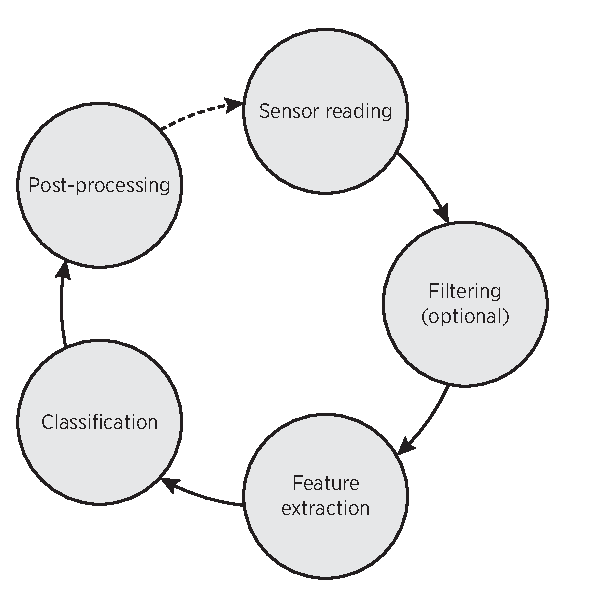
\includegraphics[width=\textwidth]{../../../resources/images/vectors/msa-stages}
  \caption{Stages of mobile sensing applications}
  \label{fig:msa-stages}
\end{figure}
\end{frame}

\begin{frame}\frametitle{Problem statement}
\begin{tcolorbox}[title=Problem statement: Mobility pattern identification,colframe=PineGreen]
\small
Given a set $V = \left\{v_{1}, v_{2}, \dotsc, v_{n}\right\}$ of data values read from sensor $S$ in the time interval $T  \in [t_{1}, t_{2}]$, identify the current mobility pattern $p_{S}$ that represents the activity of user.

\begin{equation}
  \text{PatternIdentifier}( V ) \longrightarrow{} p_{S} \in Patterns
\end{equation}

Where $Patterns$ is a set of patterns that represent an interesting state in user mobility, specifically the set $\left\{no\_movement, walking, running, vehicle\_transportation\right\}$.
\end{tcolorbox}
\end{frame}

\begin{frame}\frametitle{Problem statement}
\begin{tcolorbox}[title=Problem statement: Policy generation,colframe=PineGreen]
\small
Given the set of detected mobility patterns $\mathcal{P} = \{ p_{S_1}, p_{S_2}, \ldots, p_{S_n} \}$ in data from sensors $\mathcal{S} = \{ S_1,S_2,\ldots, S_n \}$, parameters for assigning weight to energy $e$ and accuracy $a$, and physical constraints status $c$ of a mobile device, find a policy that select the proper set of sensors $\mathcal{S}_{new}$ and its associated configuration $\mathcal{S}_{new_{conf}}$  while meeting application requirements.

\begin{equation}
  \text{PolicyGeneration}( \mathcal{P}_{\mathcal{S}}, e, a, c ) \longrightarrow{} \mathcal{S}_{new}, \mathcal{S}_{new_{conf}}
\end{equation}

The $\mathcal{S}_{new_{conf}}$ configuration is referred as the \emph{duty cycle} of associated sensor.
\end{tcolorbox}
\end{frame}

\begin{frame}\frametitle{Interaction between problems}
\begin{figure}[tb]
  \centering
  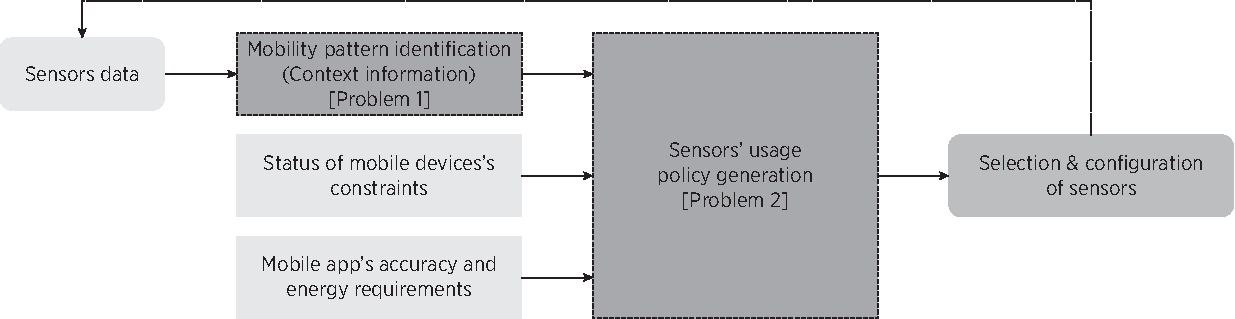
\includegraphics[width=\textwidth]{../../../resources/images/vectors/problems-incorporation}
  \caption{Interaction between the thesis work's problems}
  \label{fig:probems-incorporation}
\end{figure}
\end{frame}

\begin{frame}[t]\frametitle{Problem's scenario}
\begin{figure}[tb]
  \centering
  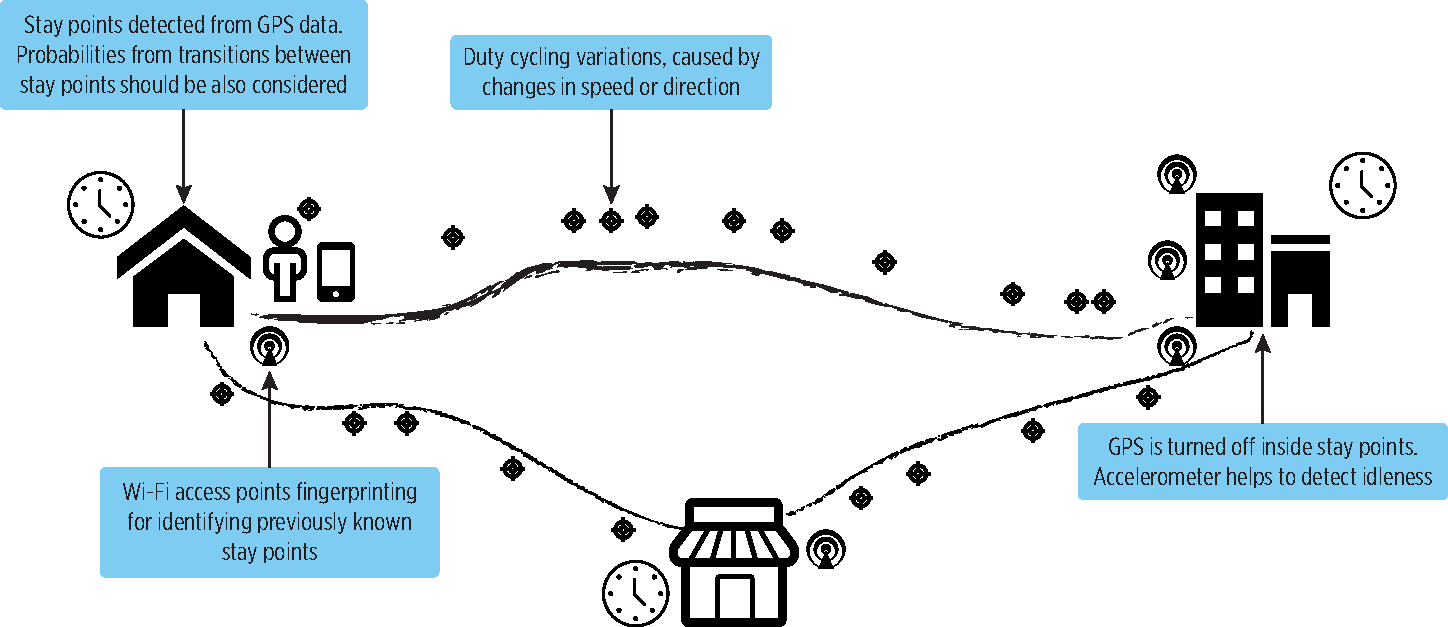
\includegraphics[width=\textwidth]{../../../resources/images/vectors/scenario}
  \caption{Basic problem's scenario}
  \label{fig:scenario}
\end{figure}
\end{frame}


\section{Methodology and current status} % Adapt your notes, this was originally separated
\subsection{Methodology and current status}
\begin{frame}[t]\frametitle{Methodology}
This is our methodology.
We can use the most updated version of the central figure.
\end{frame}

\section{State of art related techniques}
\subsection{State of art}
\begin{frame}[t]\frametitle{State of art related techniques}
A small version of the survey can fit here.
Here we have to describe the taxonomy of the survey, as well as the way the context information is prepared for adapting sensory operations (the granularity of information of the implicit second taxonomy).
We can describe works using these categories, avoiding a literal, cumbersome and too-long description of individual solutions.
\end{frame}

\begin{frame}\frametitle{Taxonomy of state of art solutions}
\begin{figure}[tb]
  \centering
  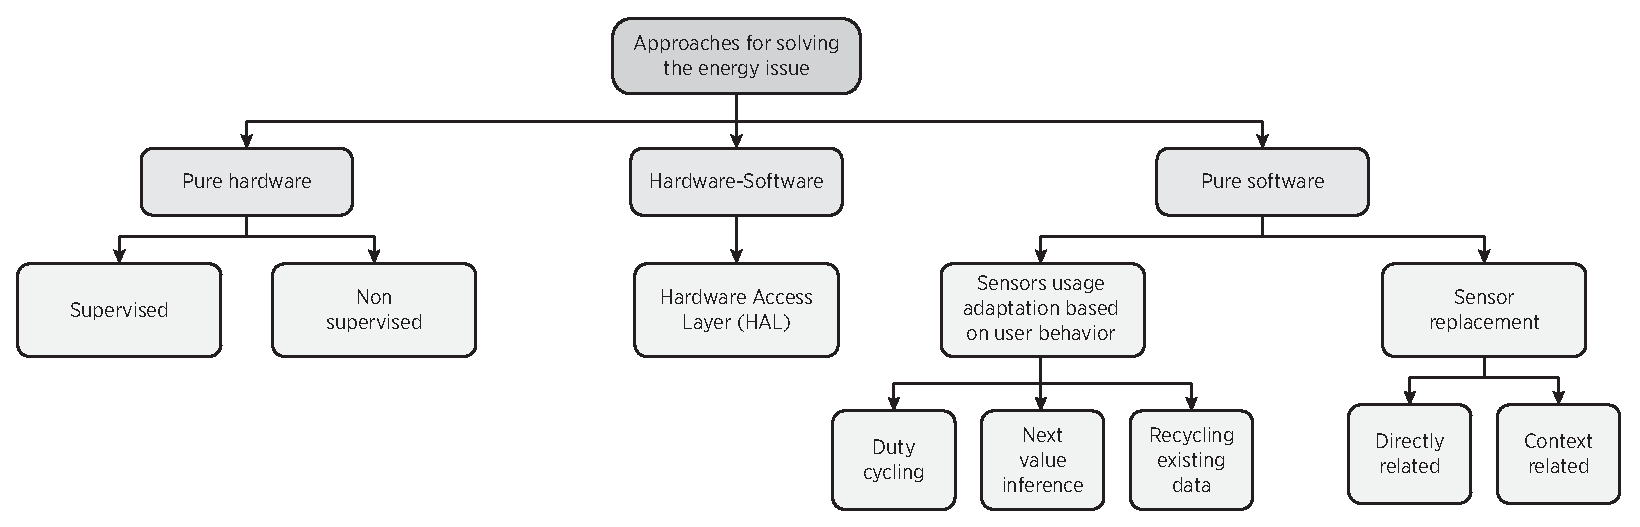
\includegraphics[width=\textwidth]{../../../resources/images/vectors/approaches-taxonomy}
  \caption{Taxonomy of solutions}
  \label{fig:taxonomy}
\end{figure}
\end{frame}

\begin{frame}\frametitle{Distribution of approaches}
\begin{figure}[tb]
  \centering
  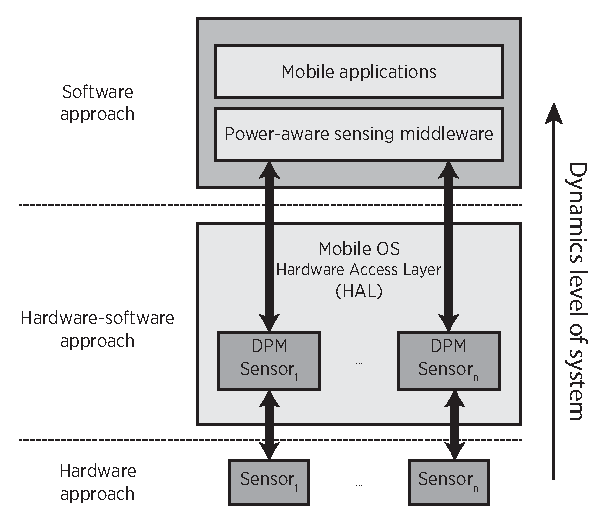
\includegraphics[scale=0.72]{../../../resources/images/vectors/approaches-distribution}
  \caption{Distribution of approaches across mobile platform's layers}
  \label{fig:distribution}
\end{figure}
\end{frame}


\section{Proposed solution}
\subsection{Proposed solution}
\begin{frame}[t]\frametitle{Proposed solution}
Figure of \emph{dual-taxonomy}.

How are we going to be different?.
At the end we can describe that:
\begin{itemize}
  \item In the ML block, we are going to produce an enhanced-expanded spatial-time model by:
  \begin{itemize}
    \item Classifying accelerometer data in user activity.
    \item Obtaining context information from other sources:
    \begin{itemize}
      \item Fingerprinting, battery status.
    \end{itemize}
    \item Obtaining speed from GPS
    \item Obtaining location from GPS and WPS
  \end{itemize}
  \item In the policy block, we will try to adapt the sensing dimension spliting the problem into:
  \begin{itemize}
    \item Learning and detection of stay points (Already covered)
    \item Learning and detection (tracking) of trajectories.
  \end{itemize}
  \item In the HW adaptation bloc, we will use several variants of the PS approach.
  For instance, we will do:
  \begin{itemize}
    \item Sensor replacement, Context related (battery) and Direct related (WPS).
    \item Adapt accordingly to what is learned from user through Duty Cycling (DC) and Recycling existing Data (RD).
    Maybe we will use Next Value Inference (VI) in the policy, when we adapt under uncertainty.
    For instance, we are 80\% sure that user is running, we will proceed with caution adapting duty cycle with fine granularity, this is negotiable.
  \end{itemize}
  \item At the end, we are trying to maintain sensors within a range that allows to perform the tracking but considering the trade-off.
\end{itemize}
\end{frame}


\section{Important results}
\subsection{Important results}
\label{sub:important_results}
\begin{frame}[t]\frametitle{Results}
    


Here, we can mentioned that we have partially prooved the possibility of performing user location tracking and stay points detection using only the smartphone.
This empowers us to keep building the blocks that will complement our solution.
\end{frame}

\section{Scientific publications produced}
\subsection{Publications}
\begin{frame}[t]\frametitle{Scientific products}
I think we can menton the survey.
We need to find out whether we can describe the article related to the on-device detection of stay points, highlighting its 'event-oriented' perspective, which represent the most natural way on which smartphone-based systems for LBS should work, being proactive.
\end{frame}


\section{Future work}
\subsection{Future work}
\begin{frame}[t]\frametitle{Future work}
    
Adequate the calendar-schedule explaining the apparent delay produced by the survey, but remarking its added value as a metric and as a scientific booster for improving the work.
\end{frame}


\section{Conclusions}
\subsection{Conclusions}
\label{sub:conclusions}
\begin{frame}[t]\frametitle{Conclusions}
Conclusions should be focused on the presentation
\end{frame}


\end{document}
